\documentclass[12pt,letterpaper]{article}
 
% --- PAQUETES NECESARIOS ---
\usepackage[utf8]{inputenc}
\usepackage[T1]{fontenc}
\usepackage[spanish,es-tabla]{babel} % Idioma español
\usepackage[margin=2.5cm]{geometry}  % Márgenes
\usepackage{graphicx}                % Para insertar imágenes
\usepackage{amsmath,amssymb}         % Símbolos matemáticos
\usepackage{setspace}                % Interlineado
\usepackage{cite}                    % Manejo de citas bibliográficas
\usepackage{listings}
\usepackage{xcolor}
\usepackage{hyperref}
\usepackage{booktabs}
\usepackage{caption}
 

\newcommand{\pend}[1]{\textcolor{red}{\textbf{[#1]}}}
 
% ===================== Estilo para bloques SQL =====================
\definecolor{codebg}{RGB}{245,245,245}
\definecolor{codekw}{RGB}{0,0,180}
\definecolor{codecomment}{RGB}{100,100,100}
 
\lstdefinelanguage{SQL}{
    keywords={SELECT, FROM, WHERE, GROUP, BY, ORDER, HAVING, AS, CREATE, TABLE, VIEW,
    INSERT, INTO, VALUES, DISTINCT, COUNT, MIN, MAX, SUM, CASE, WHEN, THEN, ELSE, END,
    CAST, DOUBLE, ASC, DESC, DROP, INSTALL, LOAD, WITH, TEMP, LIMIT, ROUND, AVG, MEDIAN,
    STDDEV, quantile_cont, generate_series, random, setseed, COPY, TO, HEADER, DELIMITER,
    FILTER, OR, AND},
    keywordstyle=\color{codekw}\bfseries,
    comment=[l]{--},
    commentstyle=\color{codecomment}\itshape,
    morestring=[b]',
    stringstyle=\color{teal},
    sensitive=false
}
 
\lstset{
    language=SQL,
    backgroundcolor=\color{codebg},
    basicstyle=\ttfamily\small,
    breaklines=true,
    frame=single,
    numbers=left,
    numberstyle=\tiny,
    xleftmargin=1.5em,
    showstringspaces=false,
    literate={á}{{\'a}}1 {é}{{\'e}}1 {í}{{\'i}}1 {ó}{{\'o}}1 {ú}{{\'u}}1
             {Á}{{\'A}}1 {É}{{\'E}}1 {Í}{{\'I}}1 {Ó}{{\'O}}1 {Ú}{{\'U}}1 {ñ}{{\~n}}1
}
 
\onehalfspacing % Interlineado de 1.5
 
\begin{document}
 
% =========================================================
% PORTADA INSTITUCIONAL
% =========================================================
\begin{titlepage}
    \centering
 
    % --- ENCABEZADO CON LOGOS ---
    \begin{minipage}{0.45\textwidth}
        \begin{flushleft}
            
\includegraphics[height=1.8cm]{imagenes/logo_tecnm.png}
        \end{flushleft}
    \end{minipage}
    \hfill
    \begin{minipage}{0.45\textwidth}
        \begin{flushright}
            
\includegraphics[height=1.8cm]{imagenes/logo_itc.png}
        \end{flushright}
    \end{minipage}
 
    \vspace{1cm}
 
    % --- INSTITUCIÓN ---
    {\bfseries\large TECNOLÓGICO NACIONAL DE MÉXICO} \\[0.3cm]
    {\bfseries\large INSTITUTO TECNOLÓGICO DE CUAUTLA} \\[0.8cm]
 
    % --- PROGRAMA Y SEMESTRE ---
    {\bfseries\large INGENIERÍA EN SISTEMAS COMPUTACIONALES} \\[0.2cm]
    {\bfseries\large ESPECIALIDAD INTELIGENCIA DE NEGOCIOS Y CIENCIA DE DATOS} \\[0.2cm]
    {\bfseries\large SÉPTIMO SEMESTRE} \\[0.8cm]
 
    % --- PERIODO Y MATERIA ---
    {\bfseries AGOSTO - DICIEMBRE 2026} \\[0.2cm]
    {\bfseries INFORME TÉCNICO - UNIDAD 2} \\[0.8cm]
 
    % --- TÍTULO DE LA ACTIVIDAD / PROYECTO ---
    {\bfseries\Large PROYECTO INTEGRADOR UNIDAD 2} \\[0.3cm]
    {\bfseries\large SIMULACIÓN Y DIAGNÓSTICO DE TRÁFICO DE RED Y LATENCIA EN SERVIDORES MEDIANTE DUCKDB Y EXCEL} \\[1.2cm]
 
    % --- PRESENTADO POR ---
    {\small PRESENTADO POR:} \\[0.1cm]
    {\bfseries KEREN SARAI VILLANUEVA LOPEZ} \\[0.6cm]
 
    % --- DOCENTE ---
    {\small DOCENTE:} \\[0.1cm]
    {\bfseries ARÍSTIDES CABALLERO ALFARO} \\[0.6cm]
 
    % --- LUGAR Y FECHA ---
    \vfill
    {\bfseries CUAUTLA, MORELOS, MÉXICO} \\
    {\bfseries OCTUBRE, 2026}
 
\end{titlepage}
 
% =========================================================
% ÍNDICES
% =========================================================
\newpage
\pagenumbering{roman} % Numeración romana para los índices

\tableofcontents % Índice General
\newpage

\listoffigures % Índice de Figuras
\newpage
 
% =========================================================
% CUERPO DEL DOCUMENTO
% =========================================================
\pagenumbering{arabic}
 
\section{Introducción}
En la operación de servicios web, la latencia de respuesta es uno de los indicadores más importantes de la calidad del servicio: un servidor puede responder de forma estable durante largos periodos y, de pronto, mostrar valores muy superiores al resto debido a bloqueos de memoria, picos de tráfico o ataques de denegación de servicio. Detectar esos valores atípicos de manera objetiva y automatizada es una tarea central del análisis exploratorio de datos. \cite{tukey-1977}
 
El presente informe documenta el desarrollo del Proyecto Integrador de la Unidad 2: \textit{Estadística Descriptiva y Exploratoria}, de la asignatura Análisis y Exploración de Datos (INC-2505). El proyecto abarca las medidas de tendencia central y dispersión, la visualización de datos para análisis exploratorio y la identificación de patrones y anomalías. Como herramientas se utilizaron \textbf{DuckDB}, un motor analítico (OLAP) embebido que se ejecuta con SQL \cite{raasveldt-2019}, para simular la telemetría, calcular las métricas y detectar anomalías, y \textbf{Microsoft Excel} para construir el diagrama de caja y bigotes que valida visualmente los resultados.
 
\section{Objetivos de la actividad}
\subsection{Objetivo general}
Caracterizar el comportamiento de la latencia de un servidor web a partir de un conjunto de datos sintético de 100 peticiones, calculando medidas de tendencia central y dispersión, detectando anomalías mediante la Regla de Tukey (IQR) en SQL y validando los resultados con un diagrama de caja y bigotes en Excel.
 
\subsection{Objetivos específicos}
\begin{itemize}
    \item Generar telemetría sintética con funciones aleatorias de DuckDB, con 95\,\% de peticiones en patrón normal (35 a 65 ms) y 5\,\% de anomalías de latencia alta (120 a 250 ms).
    \item Calcular la media, mediana, desviación estándar, mínimo, máximo, cuartiles y rango intercuartílico (IQR) mediante funciones de agregación nativas.
    \item Implementar un algoritmo SQL con expresiones de tabla comunes (CTE) que clasifique cada petición como patrón normal o anomalía.
    \item Exportar el conjunto de datos a formato CSV y construir un diagrama de caja y bigotes en Excel para contrastar visualmente la clasificación obtenida en SQL.
\end{itemize}
 
\section{Marco teórico}
 
\subsection{Medidas de tendencia central y dispersión}
Las medidas de tendencia central resumen en un solo valor el centro de un conjunto de datos. La \textbf{media aritmética} se define como
\begin{equation}
    \bar{x} = \frac{1}{n}\sum_{i=1}^{n} x_i ,
\end{equation}
y utiliza todos los valores de la muestra, por lo que es sensible a los valores extremos. La \textbf{mediana} es el valor que divide a los datos ordenados en dos mitades iguales; depende de la posición y no de la magnitud de los extremos, por lo que es una medida robusta. \cite{tukey-1977}
 
Entre las medidas de dispersión se encuentra la \textbf{desviación estándar muestral},
\begin{equation}
    s = \sqrt{\frac{1}{n-1}\sum_{i=1}^{n}(x_i-\bar{x})^2},
\end{equation}
que cuantifica qué tan alejados están los datos de la media y, al elevar al cuadrado las diferencias, también es sensible a valores atípicos. Los \textbf{cuartiles} $Q_1$, $Q_2$ (mediana) y $Q_3$ dividen la distribución en cuatro partes con igual número de observaciones, y el \textbf{rango intercuartílico} (IQR) es
\begin{equation}
    \mathrm{IQR} = Q_3 - Q_1,
\end{equation}
que describe la amplitud del 50\,\% central de los datos y es robusto ante valores extremos. En DuckDB, la función \texttt{quantile\_cont} calcula cuantiles con interpolación lineal. \cite{duckdb-docs}
 
\subsection{Visualización de datos para análisis exploratorio}
El diagrama de caja y bigotes (\textit{boxplot}), propuesto por Tukey, resume la distribución de una variable con cinco elementos: la caja, delimitada por $Q_1$ y $Q_3$; una línea interna en la mediana; los bigotes, que se extienden hasta el dato más lejano dentro de los límites de Tukey; y los puntos aislados, que representan los valores atípicos. \cite{tukey-1977} Es una herramienta apropiada para comparar de forma rápida el centro, la dispersión, la simetría y las anomalías de un conjunto de datos. Excel incorpora este tipo de gráfico entre sus gráficos estadísticos. \cite{microsoft-boxwhisker}
 
\subsection{Identificación de patrones y anomalías: Regla de Tukey}
La Regla de Tukey considera atípico a todo valor que queda fuera del intervalo
\begin{equation}
    \left[\,Q_1 - 1.5\cdot\mathrm{IQR},\; Q_3 + 1.5\cdot\mathrm{IQR}\,\right].
\end{equation}
Al basarse en cuartiles y no en la media y la desviación estándar, los límites no se distorsionan por los propios valores anómalos, lo que la hace adecuada para detectar picos de latencia. \cite{tukey-1977}
 
\subsubsection{Valores esperados del modelo de simulación}
Dado que la simulación mezcla 95\,\% de datos uniformes en $[35,65]$ con 5\,\% de datos uniformes en $[120,250]$, es posible anticipar valores teóricos de referencia para validar la ejecución:
\begin{itemize}
    \item El número de anomalías generadas sigue una distribución binomial $B(100,\,0.05)$, con valor esperado $np=5$ y desviación estándar $\sqrt{np(1-p)}\approx 2.18$; por tanto, en distintas corridas es normal obtener valores cercanos a 5 (por ejemplo, de 2 a 9).
    \item La media teórica de la mezcla es $0.95(50)+0.05(185)=56.75$ ms, mientras que la mediana teórica es aproximadamente $50.79$ ms.
    \item Los cuartiles teóricos son $Q_1\approx 42.89$ ms y $Q_3\approx 58.68$ ms, con $\mathrm{IQR}\approx 15.79$ ms, lo que produce límites de Tukey de aproximadamente $19.21$ ms (inferior) y $82.37$ ms (superior).
\end{itemize}
Como todas las anomalías simuladas ($\geq 120$ ms) superan el límite superior y todos los datos normales ($\leq 65$ ms) quedan por debajo de él, se espera que la regla clasifique exactamente como anomalía a las peticiones generadas por la rama de alta latencia.
 
\section{Herramientas utilizadas}
\begin{itemize}
    \item DuckDB CLI para la generación de datos, el cálculo de métricas y la detección de anomalías. \cite{duckdb-docs}
    \item Microsoft Excel para la construcción del diagrama de caja y bigotes.
\end{itemize}
 
\section{Desarrollo}
 
\subsection{Fase 1: Generación del conjunto de datos sintético}
Se creó una tabla temporal con 100 peticiones consecutivas. Cada petición tiene una probabilidad de 5\,\% de ser una anomalía (latencia entre 120 y 250 ms) y 95\,\% de seguir el patrón normal del servidor (entre 35 y 65 ms). Para que los resultados sean reproducibles, se fijó una semilla con \texttt{setseed}. La función \texttt{random()} genera un valor uniforme en $[0,1)$, que se utiliza para decidir si la petición es normal o anómala y para calcular la latencia correspondiente.
 
\begin{lstlisting}[caption={Generación de la telemetría sintética}]
CREATE TEMP TABLE telemetria_servidor AS
SELECT
    peticion_id,
    CASE
        WHEN random() < 0.05 THEN ROUND(120 + (random() * 130), 2)
        ELSE ROUND(35 + (random() * 30), 2)
    END AS latencia_ms
FROM generate_series(1, 100) AS t(peticion_id);
 
SELECT * FROM telemetria_servidor LIMIT 10;
\end{lstlisting}
 
\begin{figure}[h]
    \centering
    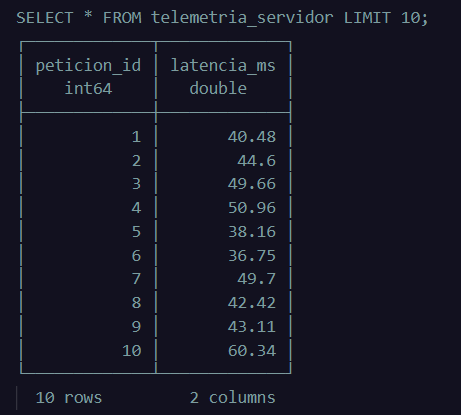
\includegraphics[width=0.5\textwidth]{imagenes/fase1_primeros_registros.png}
    \caption{Primeros 10 registros de la tabla \texttt{telemetria\_servidor}.}
    \label{fig:fase1}
\end{figure}
 
\subsection{Fase 2: Caracterización del patrón base}
Se calcularon las medidas de tendencia central y dispersión con las funciones \texttt{AVG}, \texttt{MEDIAN}, \texttt{STDDEV} y \texttt{quantile\_cont}.
 
\begin{lstlisting}[caption={Cálculo de medidas descriptivas}]
SELECT
    ROUND(AVG(latencia_ms), 2)                  AS Media,
    ROUND(MEDIAN(latencia_ms), 2)               AS Mediana,
    ROUND(STDDEV(latencia_ms), 2)               AS Desviacion_Estandar,
    ROUND(MIN(latencia_ms), 2)                  AS Minimo,
    ROUND(MAX(latencia_ms), 2)                  AS Maximo,
    ROUND(quantile_cont(latencia_ms, 0.25), 2)  AS Q1_Cuartil1,
    ROUND(quantile_cont(latencia_ms, 0.75), 2)  AS Q3_Cuartil3,
    ROUND(quantile_cont(latencia_ms, 0.75)
        - quantile_cont(latencia_ms, 0.25), 2)  AS IQR
FROM telemetria_servidor;
\end{lstlisting}
 
\begin{figure}[h]
    \centering
    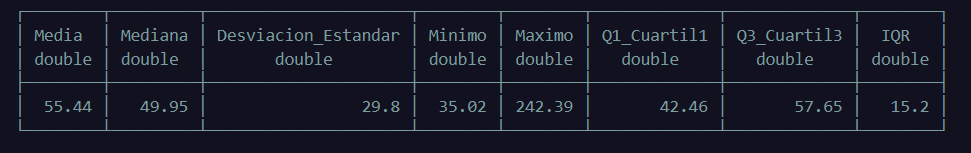
\includegraphics[width=0.9\textwidth]{imagenes/fase2_medidas.png}
    \caption{Resultado de las medidas descriptivas calculadas en DuckDB.}
    \label{fig:fase2}
\end{figure}
 
\begin{table}[h]
    \centering
    \caption{Medidas descriptivas de la latencia (ms) obtenidas en la ejecución.}
    \label{tab:descriptivas}
    \begin{tabular}{lc}
        \toprule
        \textbf{Medida} & \textbf{Valor (ms)} \\
        \midrule
        Media                & 55.44 \\
        Mediana              & 49.95 \\
        Desviación estándar  & 29.80 \\
        Mínimo               & 35.02 \\
        Máximo               & 242.39 \\
        $Q_1$                & 42.46 \\
        $Q_3$                & 57.65 \\
        IQR                  & 15.20 \\
        \bottomrule
    \end{tabular}
\end{table}
 

\subsubsection{Cuestionario reflexivo 1}
\textbf{Pregunta:} Compara el valor de la media respecto a la mediana. Explica por qué la presencia de picos de latencia desvía la media hacia un valor más alto, mientras la mediana se mantiene estable.
 
\textbf{Respuesta:} En la ejecución se obtuvo una media de 55.44 ms y una mediana de 49.95 ms, es decir, la media resultó 5.49 ms mayor. La media se calcula sumando todos los valores, de modo que una petición de, por ejemplo, 200 ms contribuye con su magnitud completa y arrastra el promedio hacia arriba, aun cuando la gran mayoría de las peticiones esté cerca de 50 ms. La mediana, en cambio, solo depende de cuál es el valor que ocupa la posición central al ordenar los datos: que un extremo valga 130 o 250 ms no cambia su posición, por lo que la mediana permanece dentro del rango normal (35 a 65 ms) y refleja el verdadero patrón central del servidor. La desviación estándar de 29.80 ms, mucho mayor que la que tendría el tráfico normal por sí solo (alrededor de 8.7 ms para una distribución uniforme entre 35 y 65), también se infla por la presencia de los picos.
 
\subsection{Fase 3: Detección automatizada de anomalías con la Regla de Tukey}
Se implementó la Regla de Tukey mediante dos CTE: \texttt{metricas}, que obtiene $Q_1$, $Q_3$ e IQR, y \texttt{limites}, que calcula los límites inferior y superior. Posteriormente, cada petición se compara contra dichos límites para asignarle un diagnóstico.
 
\begin{lstlisting}[caption={Clasificación de peticiones con la Regla de Tukey}]
WITH metricas AS (
    SELECT
        quantile_cont(latencia_ms, 0.25) AS Q1,
        quantile_cont(latencia_ms, 0.75) AS Q3,
        (quantile_cont(latencia_ms, 0.75)
         - quantile_cont(latencia_ms, 0.25)) AS IQR
    FROM telemetria_servidor
),
limites AS (
    SELECT
        Q1, Q3, IQR,
        (Q1 - 1.5 * IQR) AS limite_inferior,
        (Q3 + 1.5 * IQR) AS limite_superior
    FROM metricas
)
SELECT
    t.peticion_id,
    t.latencia_ms,
    CASE
        WHEN t.latencia_ms > l.limite_superior THEN 'ANOMALÍA (Spike Alto)'
        WHEN t.latencia_ms < l.limite_inferior THEN 'ANOMALÍA (Bajo Rango)'
        ELSE 'Patrón Normal'
    END AS diagnostico_sistema
FROM telemetria_servidor t, limites l
ORDER BY t.peticion_id;
\end{lstlisting}

\begin{figure}[h]
    \centering
    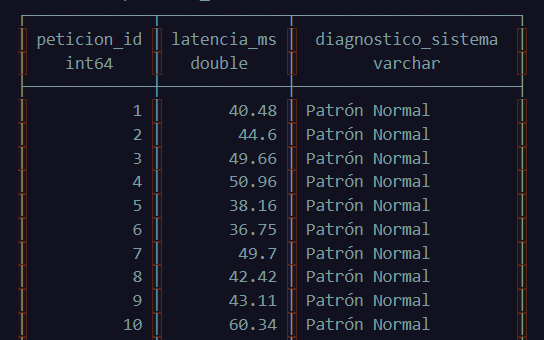
\includegraphics[width=0.7\textwidth]{imagenes/fase3_diagnostico.png}
    \caption{Clasificación de las peticiones según la Regla de Tukey.}
    \label{fig:fase3}
\end{figure}
 
Cabe señalar que en la guía original la cláusula \texttt{FROM} de la CTE \texttt{limites} aparece vacía; se corrigió a \texttt{FROM metricas}. Para responder cuántas peticiones fueron anómalas y qué umbrales se aplicaron, se agregó una consulta de conteo.
 
\begin{lstlisting}[caption={Conteo de anomalías y límites de Tukey}]
WITH m AS (
    SELECT quantile_cont(latencia_ms, 0.25) AS Q1,
           quantile_cont(latencia_ms, 0.75) AS Q3
    FROM telemetria_servidor
),
l AS (
    SELECT Q1, Q3, Q1 - 1.5*(Q3-Q1) AS lim_inf,
           Q3 + 1.5*(Q3-Q1) AS lim_sup
    FROM m
)
SELECT
    ROUND(l.lim_inf, 2) AS limite_inferior,
    ROUND(l.lim_sup, 2) AS limite_superior,
    COUNT(*) FILTER (WHERE t.latencia_ms > l.lim_sup) AS anomalias_spike_alto,
    COUNT(*) FILTER (WHERE t.latencia_ms < l.lim_inf) AS anomalias_bajo_rango,
    COUNT(*) FILTER (WHERE t.latencia_ms > l.lim_sup
                        OR t.latencia_ms < l.lim_inf) AS total_anomalias
FROM telemetria_servidor t, l
GROUP BY l.lim_inf, l.lim_sup;
\end{lstlisting}
 
\begin{figure}[h]
    \centering
    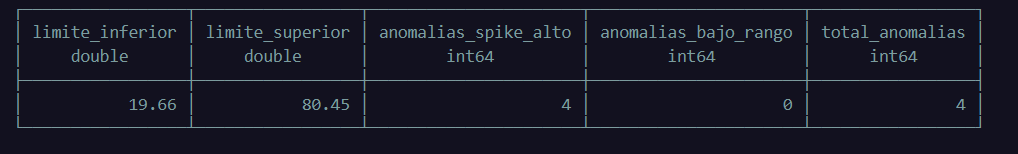
\includegraphics[width=0.9\textwidth]{imagenes/fase3_conteo.png}
    \caption{Límites de Tukey y conteo total de anomalías.}
    \label{fig:fase3conteo}
\end{figure}
 
Los límites obtenidos fueron $[\,19.66\,,\,80.45\,]$ ms, y se identificaron 4 peticiones anómalas, todas ellas de tipo \textit{Spike Alto}. La Tabla~\ref{tab:anomalias} lista las peticiones detectadas.
 
\begin{table}[h]
    \centering
    \caption{Peticiones clasificadas como anomalía (Spike Alto).}
    \label{tab:anomalias}
    \begin{tabular}{cc}
        \toprule
        \textbf{peticion\_id} & \textbf{latencia\_ms} \\
        \midrule
        83 & 242.39 \\
        66 & 183.33 \\
        33 & 177.43 \\
        61 & 162.86 \\
        \bottomrule
    \end{tabular}
\end{table}
 
\subsection{Fase 4: Exportación y validación gráfica en Excel}
Los datos se exportaron a un archivo CSV con el siguiente comando:
 
\begin{lstlisting}[caption={Exportación de la tabla a CSV}]
COPY telemetria_servidor TO 'telemetria_servidor.csv' (HEADER, DELIMITER ',');
\end{lstlisting}
 
El archivo resultante contiene dos columnas: \texttt{peticion\_id} (columna A) y \texttt{latencia\_ms} (columna B). Por ello, para el diagrama se seleccionó el rango \textbf{B1:B101}, que corresponde a la latencia, y no A1:A101 como indicaba la guía. Posteriormente se utilizó \textit{Insertar $\rightarrow$ Gráficos estadísticos $\rightarrow$ Caja y bigotes}, se activó la opción de mostrar puntos atípicos y el cálculo de cuartiles con mediana inclusiva (equivalente a la interpolación de \texttt{quantile\_cont}), y se configuraron el título del gráfico y los títulos y escala del eje vertical.
 
\begin{figure}[h]
    \centering
    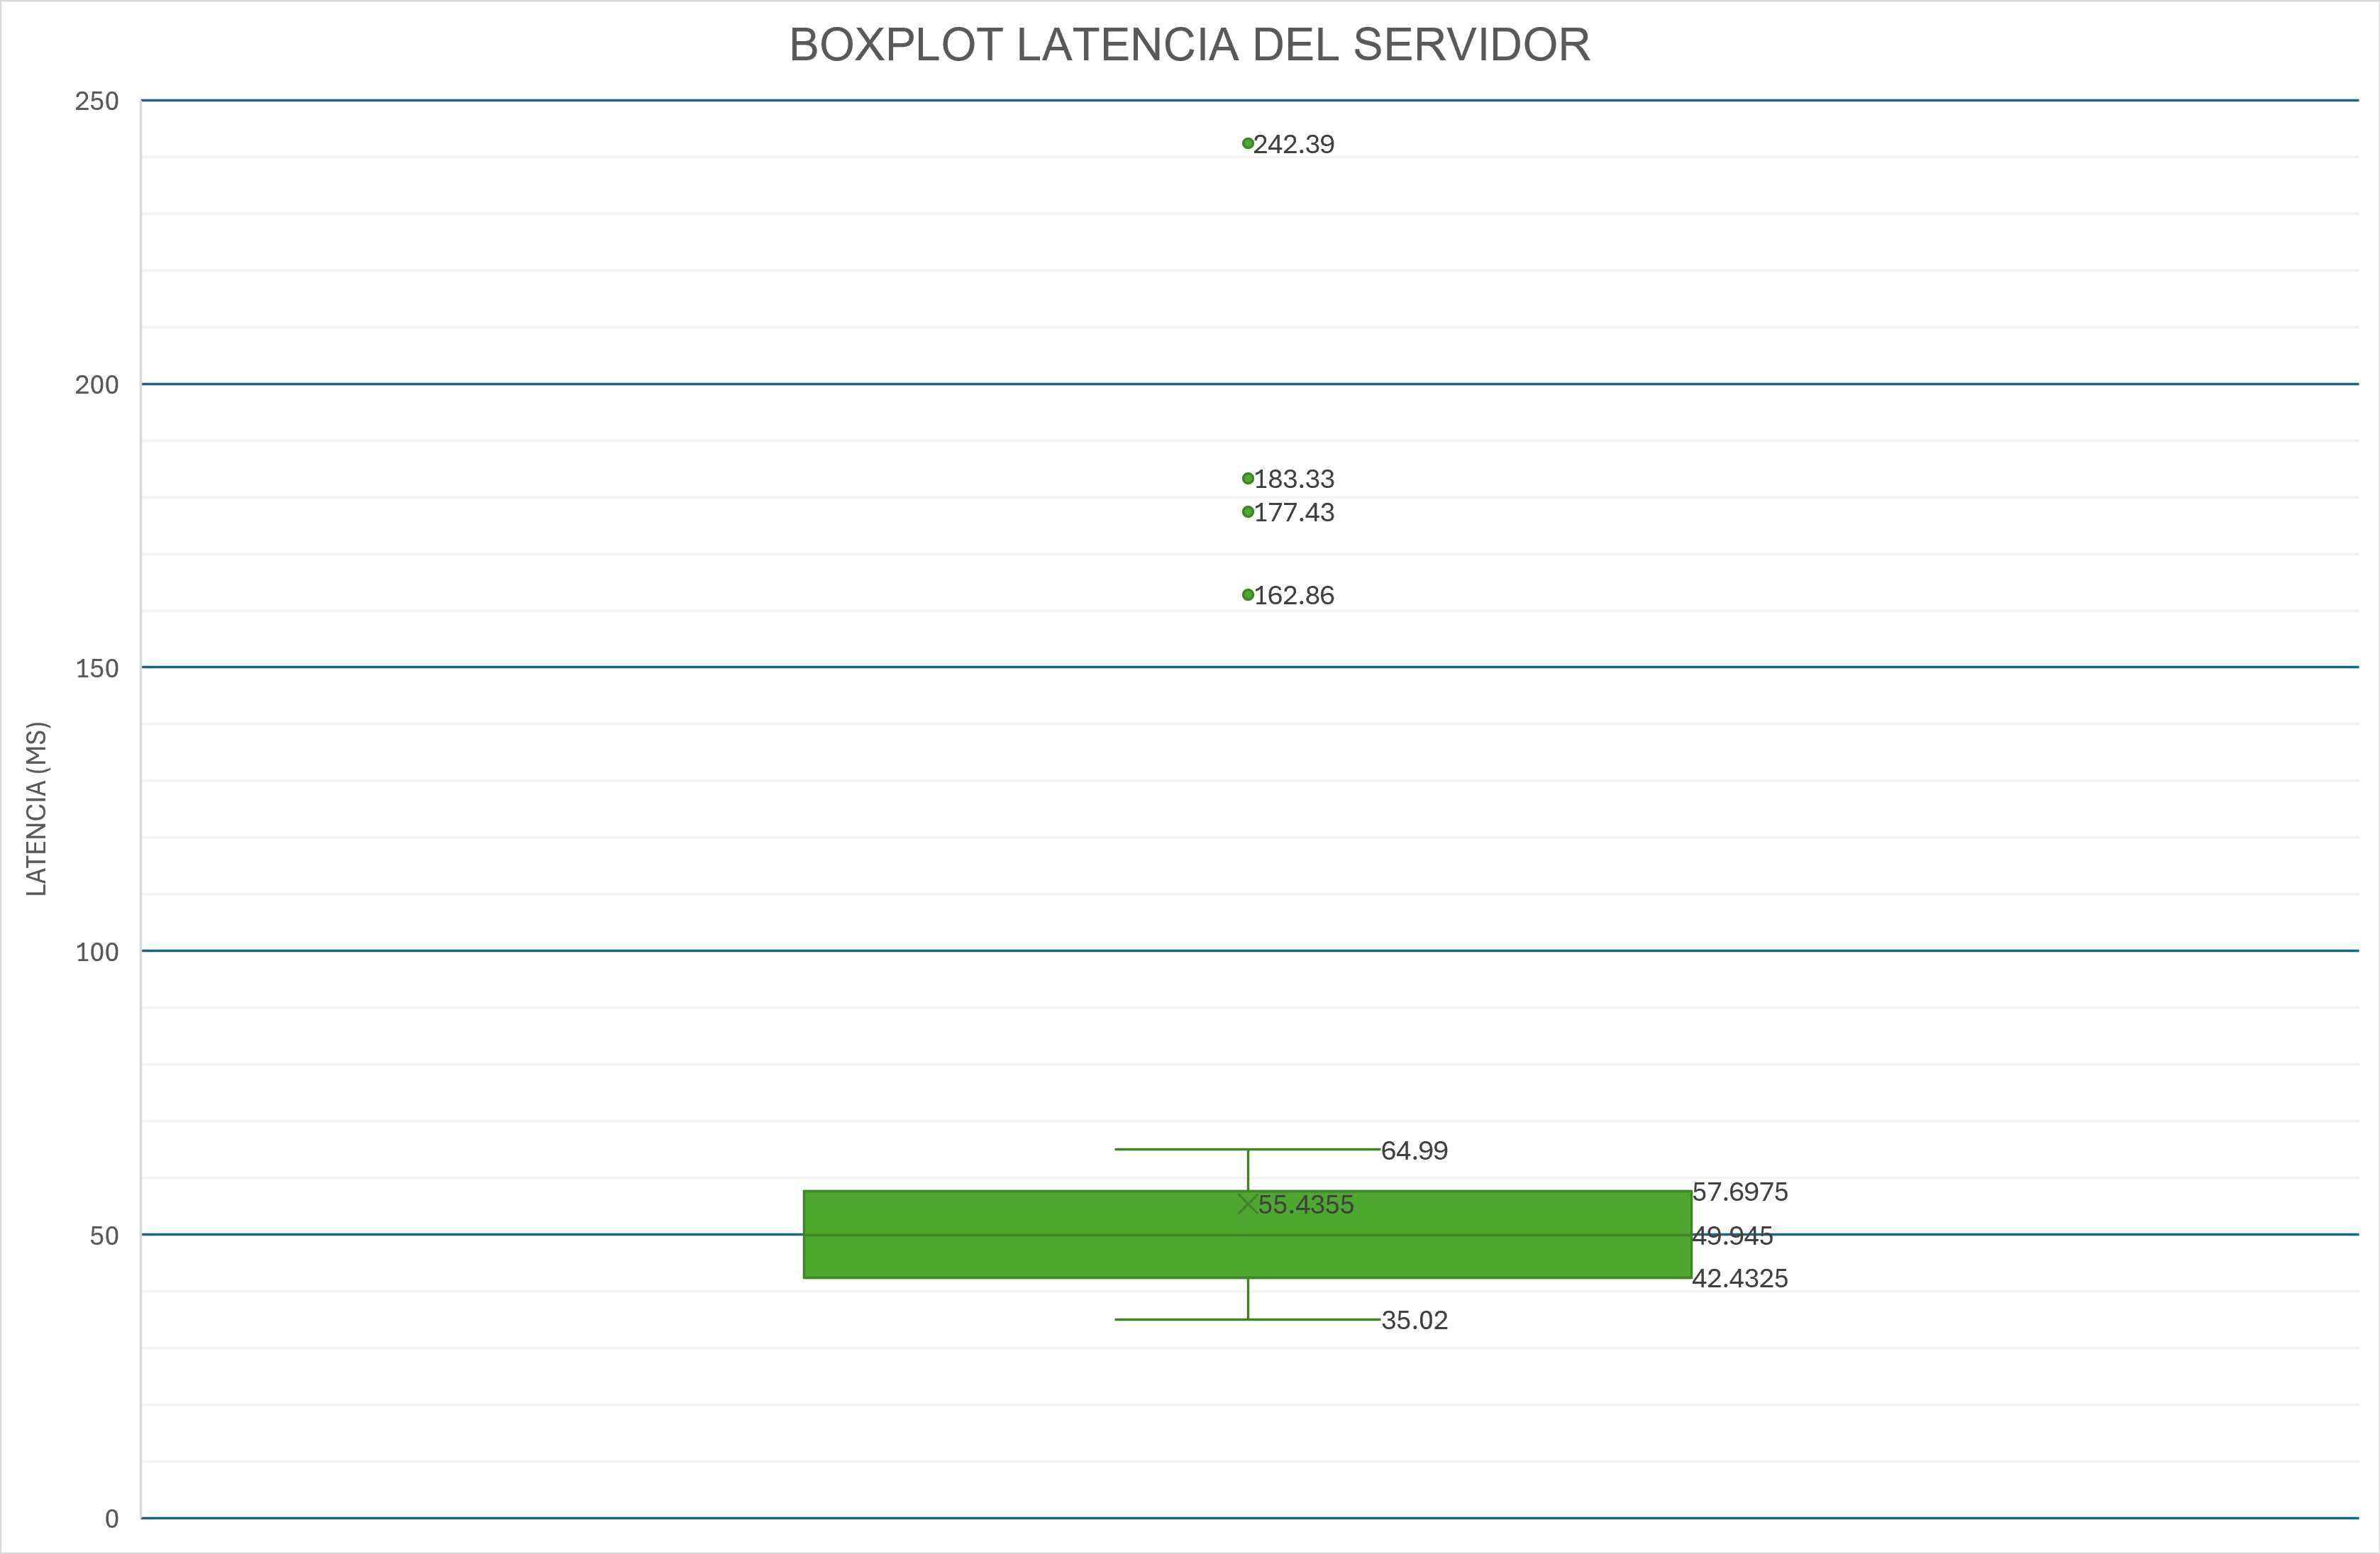
\includegraphics[width=1.0\textwidth]{imagenes/boxplot_excel.png}
    \caption{Diagrama de caja y bigotes de la latencia del servidor generado en Excel.}
    \label{fig:boxplot}
\end{figure}
 
\textbf{Validación:} en la Figura~\ref{fig:boxplot} se observa que las 4 peticiones clasificadas en SQL como \textit{ANOMALÍA (Spike Alto)} aparecen como puntos aislados por encima del bigote superior, mientras que el resto de las peticiones queda contenido dentro de la caja y los bigotes. El bigote superior termina en aproximadamente 64.99 ms, valor coherente con el dato normal más alto y con el límite superior de 80.45 ms calculado en SQL. Esto confirma que el algoritmo SQL y la herramienta gráfica aplican el mismo criterio.
 
\subsection{Registro de comandos (log)}
Para cumplir con el entregable, la salida del CLI de DuckDB se redirigió a un archivo de texto al ejecutar el script del proyecto.
 
\begin{lstlisting}[caption={Generación del log de comandos}]
-- Opcion 1: ejecutar todo el script y guardar la salida
--   duckdb < proyecto_u2.sql > log_comandos_23680116_U2.txt
 
-- Opcion 2: dentro del CLI
.output log_comandos_23680116_U2.txt
.echo on
-- ... ejecutar las fases 1 a 4 ...
.output stdout
\end{lstlisting}
 
El archivo generado, \texttt{log\_comandos\_23680116\_U2.txt}, se adjunta como entregable independiente, junto con el PDF del diagrama de caja y bigotes.
 
\begin{figure}[h]
    \centering
    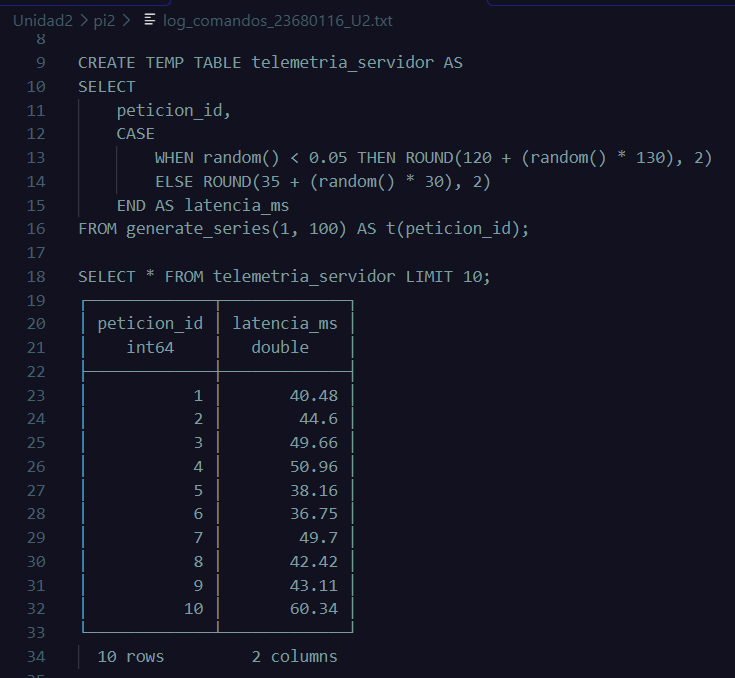
\includegraphics[width=0.5\textwidth]{imagenes/log_comandos.png}
    \caption{Fragmento del log de comandos generado por DuckDB.}
    \label{fig:log-comandos}
\end{figure}
 
\section{Conclusiones de ingeniería}
 
\subsection{¿Cuántas peticiones fueron clasificadas como anomalías en total?}
Se clasificaron 4 de las 100 peticiones como anomalías, es decir, el 4\,\% de la muestra, todas de tipo \textit{Spike Alto}. Este resultado es consistente con el modelo de simulación: como cada petición tiene 5\,\% de probabilidad de ser anómala, el número esperado es de 5 con una desviación estándar de aproximadamente 2.2, por lo que variaciones entre corridas son normales.
 
\subsection{¿Qué representa el rango intercuartílico (IQR) en el análisis del rendimiento del servidor?}
El IQR, que en esta ejecución fue de 15.20 ms, representa la amplitud del 50\,\% central de las latencias; es decir, qué tanto varía el tiempo de respuesta durante la operación típica del servidor, sin influencia de los picos. Un IQR pequeño indica un servicio estable y predecible; un IQR grande, un servicio irregular. Además, el IQR define los umbrales de la Regla de Tukey, de modo que el criterio de anomalía se adapta al comportamiento real del servidor en lugar de depender de un valor fijo arbitrario, y no se contamina con los propios picos que busca detectar, a diferencia de un criterio basado en la media y la desviación estándar.
 
\subsection{¿Qué acciones de infraestructura se recomiendan si este servidor estuviera en producción?}
\begin{itemize}
    \item \textbf{Monitoreo y alertas:} vigilar percentiles altos (p95 y p99) y configurar alertas automáticas cuando la latencia supere el límite de Tukey calculado sobre una ventana móvil, en lugar de basarse solo en el promedio.
    \item \textbf{Escalamiento y balanceo de carga:} implementar autoescalado horizontal y balanceadores de carga para absorber picos legítimos de tráfico.
    \item \textbf{Protección contra ataques:} aplicar limitación de tasa (\textit{rate limiting}), un firewall de aplicaciones web y servicios de mitigación de denegación de servicio.
    \item \textbf{Diagnóstico de memoria:} revisar el uso de memoria y el recolector de basura para identificar fugas o bloqueos que expliquen picos aislados.
    \item \textbf{Tolerancia a fallos:} usar caché, \textit{timeouts} y \textit{circuit breakers} para evitar que una petición lenta se propague a otros servicios.
    \item \textbf{Mejora continua:} realizar pruebas de carga periódicas y mantener un procedimiento documentado de respuesta a incidentes, registrando la causa de cada anomalía detectada.
\end{itemize}
 
\subsection{Conclusión general}
Este proyecto permitió integrar los tres temas de la unidad: las medidas descriptivas dieron el patrón base del servidor, la visualización con el diagrama de caja y bigotes permitió ver de un vistazo la dispersión y los valores extremos, y la Regla de Tukey convirtió esa intuición visual en un criterio automatizable en SQL. Una enseñanza central fue la diferencia entre medidas sensibles (media y desviación estándar) y medidas robustas (mediana e IQR) ante valores atípicos: las segundas describen mejor el comportamiento normal, y las primeras sirven, precisamente, para evidenciar que algo anómalo ocurrió. También quedó clara la utilidad de contrastar un resultado obtenido por cálculo con una representación gráfica independiente, ya que ambas coinciden en confirmar el diagnóstico y ayudan a detectar errores, como los dos que se corrigieron en la guía original (la cláusula \texttt{FROM} vacía y el rango de columna).
 
% =========================================================
% BIBLIOGRAFÍA
% =========================================================
\newpage
 
\bibliographystyle{ieeetr}
\bibliography{referencias}
 
\end{document}
 
